\documentclass[a4paper]{article}
\usepackage[utf8]{inputenc}
\usepackage[T1]{fontenc}
\usepackage{graphicx}
\usepackage{hyperref}
\usepackage[english]{babel}
\usepackage{url}
\usepackage[super]{nth}
\usepackage{fancyhdr}
\usepackage{tabu}


\DeclareGraphicsExtensions{.pdf,.png,.jpg,.eps}

\newcommand{\myauthor}{TODO Names of Authors}
\newcommand{\mytitle}{Zombie Apocalypse Report}

\lhead{\mytitle}
\rhead{\myauthor}

\pagestyle{fancy}
\fancyhf{}
\fancyhead[L]{TODO names of authors}
\fancyhead[R]{\mytitle}

\fancyfoot[C]{\thepage}

\title{\mytitle}
\author{\myauthor}

\begin{document}
\maketitle

\section{Introduction} % Ryan

\section{Model} % Adam

\subsection{Infection model}

\begin{figure*}[ht]
        \centering
        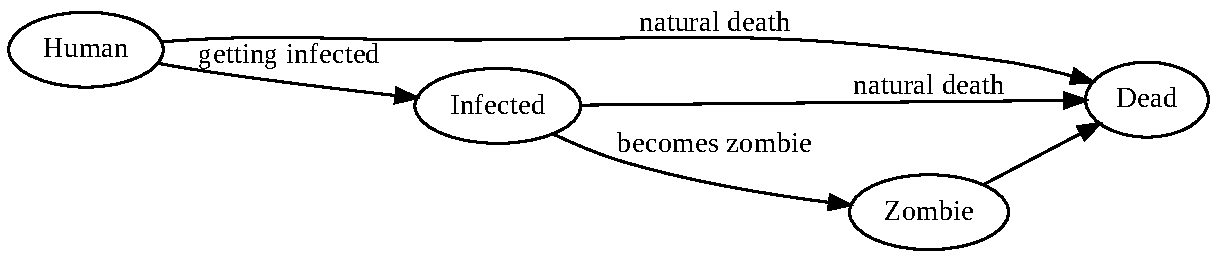
\includegraphics[width=\textwidth]{model}
        \caption{Infection model}
\end{figure*}

Since there has not been found cure for zombies to become humans, our model presumes only four possible stages.
An entity begins in state Human which represent a normal human being which was born, has a gender (is either male of female) and eventually dies.
If a human gets in contact with a zombie, it may become infected.
Infected entity is basically a human which eventually becomes a zombie which means that it can reproduce and die of natural death.
Infected entity is not a danger to the surrounding humans until it becomes a zombie.
When in contact with a human, a zombie may infect him or her.
Zombie is concidered death -- it is just a virus driven moving body; therefore we say that a zombie eventually decomposes insead of it dies.
In our model, zombie doesn't have gender as it cannot reproduce nor its properties depend on gender of the human which it used to be.

When a human becomes infected, the length of the infection is determined by the strength of the body fighting zombie virus.
The virus seems to be latent once a day it tries to gain control over the body.
It will happen with a certain probability.

\subsubsection{Reproduction}

If two fertile living entities (no matter if human or infected) of different genders meet, they can make love and conceive a child or children.
It takes approximately 9 months for the children to develop inside mother's womb before they are born.
As the zombies are of viral nature, we presume that the virus in infected mother's body is passed to unborn children.
The virus is not transmitted when an infected has an intercourse with a human.

A woman can become pregnat if she is not already pregnant and she is an a fertile age (roughtly between 15 and 45 years) and her partner is a male in a fertile age (roughtly between 15 and 80).
More than one baby can be conceived during one intercourse -- our model supports that a female can have up to three children at once.
The probabilities of multiple births are in accordance with Hellin's law. (TODO reference)

\subsubsection{Age}

The model follows the Australian age distribution for both males and females.
When the simulation starts, the people are didided into age classes based on their gender.
Within the age class the people are distributed uniformly.

Humans and infected are sorted into four age classes:
\begin{enumerate}
\item a child (0 -- 15 years)
\item young (15 -- 37.5 years)
\item middle aged (37.5 -- 65 years)
\item elderly (54 -- $\infty$)
\end{enumerate}

According to latest scientific research (TODO reference), zombies live 3 to 5 years. 
Zombies are divided into two age classes:
\begin{enumerate}
\item young (0 -- 1.5 years)
\item old (1.5 -- $\infty$)
\end{enumerate}

Most of the properties of the entities are dependent on their age class rather than on their actual age.
Those properties are:
\begin{itemize}
\item daily death rate -- probability of natural death per each day
\item speed -- probability of entity to leave current tile if it was its original intension
\end{itemize}

We have good estimates for living entities, but we are still waiting for our colleagues to determine the values for zombies depending on their age.

\subsection{World representation}

The simulated world is a mesh of size $1000 \times 1500$ which correspond with size of Northern Territory. (TODO reference)
Parts of the mesh are called tiles.
On each tile, there may be at most one entity of any type.
Adjacency of two entities means that the two entities are touching each other, sharing one side of their tiles.
The simulated world has fixed boundaries and no entity can pass through them; this is often refered as no-flux boundary. (TODO reference)

For the purpose of this report, only part of the world is simulated.
The actual size of the mesh is $500 \times 500$ tiles.

\subsubsection{Movement}

\begin{figure*}[ht]
    \centering
    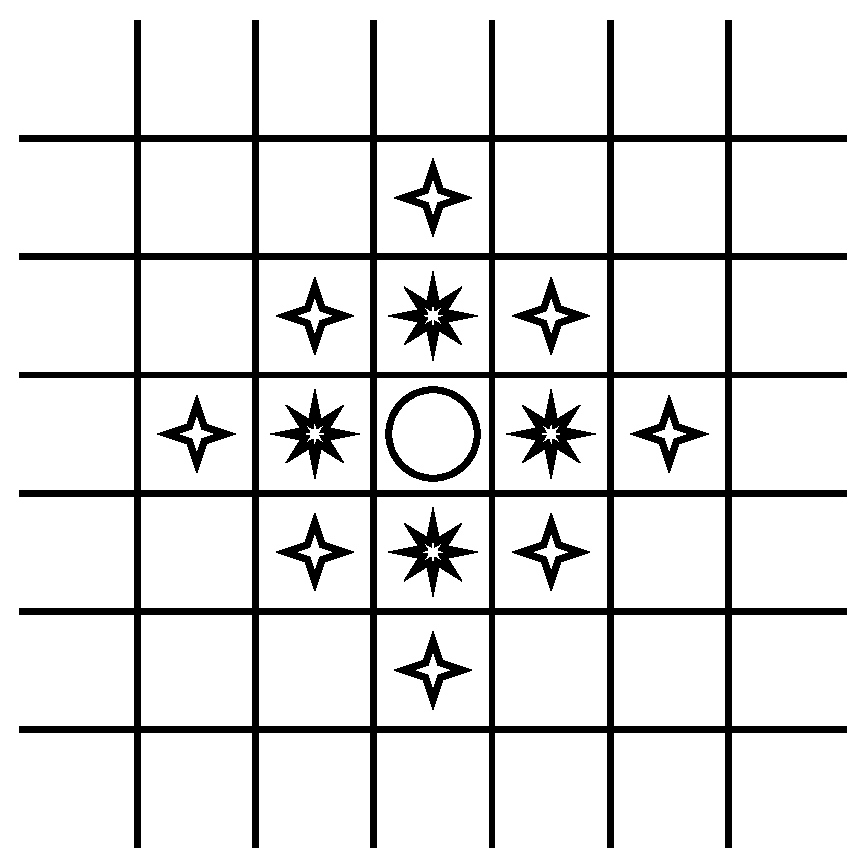
\includegraphics[width=0.3\textwidth]{movement}
    \caption{Considered tiles when planning movement}
\end{figure*}

\begin{figure*}[ht]
    \centering
    \begin{tabu} {| X[1.8,c,p] || X[1,c,p] | X[1,c,p] | X[1,c,p] | X[1,c,p] | X[1.2,c,p] |}
        \rowfont{\bfseries}
        \hline
        sees &
        Wall &
        Empty tile&
        Zombie &
        Same gender &
        Opposite gender \\
        \hline
        \hline
        \textbf{Living entity} & -- & + & -- & + & ++ \\
        \hline
        \textbf{Zombie} & -- & + & + & \multicolumn{2}{c|}{ ++ } \\
        \hline
    \end{tabu}
    \caption{Affinity to directed situations for each type}
\end{figure*}


All entities share the same intelligence, even zombies.
They differ mainly in preference where to go.

Each entity determines its optimal direction based on surrounding 12 tiles as shown on the diagram.
The tiles which it can get within one move are marked with a fancy star; tiles accessible within two moves are marked with a simple star.
The adjacent tiles always have higher priority.

Each living entity and zombie rate each of these tiles based on their content.
The preference for direction is then calculated as a weighted sum of complex numbers corresponding to direction.
The exact values of preferences may change as soon as we obtain a broader set of observations of entities in various situations.
However the estimates can be seen in the table.
To the current preffered direction the direction from the last move is added, which simulates inertia of movement and as a result it makes the movement targeted.

After the optimal weighted direction is calculated, it is translated to a direction or stay instruction if the absolute value is not sufficient.
The direction may randomly change clock-wise or counter-clock-wise simulating evading obstacles, which are not modeled in the world.
Then the tile in resulting direction is tested whether it is free; if it is not, the clock-wise or cunter-clock-wise is chosen.
In the worst case, the entity stays at its current tile.
The entity moves only if its speed (expressed as probability) is sufficient.

\subsubsection{Stability}

TODO Alicia will describe her magic

\section{Results}

TODO two images of state and a graph of populations' count.

\section{Recommendations}

TODO we should add bibliography to the end

\end{document}

% vim: ft=tex ts=4 sw=4 et
